\section{Problem Formulation and Botanical Foliar Archetypes}
\label{sec:problem_formulation}

\subsection{Episodic Few-Shot Formulation}
\label{subsec:few_shot_formulation}
We formulate autonomous in-the-wild crop disease diagnosis within an episodic $N$-way $K$-shot metric learning framework. Let $\mathcal{X} \subset \mathbb{R}^{H \times W \times 3}$ denote the natural image space and $\mathcal{Y} = \{1, 2, \dots, C\}$ denote the label space comprising $C$ fine-grained crop pathology categories. In each diagnostic episode instantiated from task distribution $\mathcal{T}$, the system receives a labeled support set $\mathcal{S} = \bigcup_{c=1}^N \{(x_{c,k}, y_{c,k})\}_{k=1}^K$ containing $K$ exemplars per class ($K=5, |\mathcal{S}| = N \times K$), and an unlabelled query set $\mathcal{Q} = \{(x_j^q, y_j^q)\}_{j=1}^{|\mathcal{Q}|}$ evaluating generalization across unseen field leaves.

Standard metric few-shot learning computes a class prototype vector $P_c = \frac{1}{K}\sum_{x \in \mathcal{S}_c} f_\theta(x)$ via a deep backbone $f_\theta: \mathcal{X} \to \mathbb{R}^D$, assigning query predictions by nearest Euclidean distance: $\hat{y}^q = \arg\min_c \|f_\theta(x^q) - P_c\|_2$. Under real-world agricultural conditions, however, standard metric prototypes break down due to two interrelated phenomena: (i) scaling $N$ across dozens of pathologies induces severe metric overlap between visually similar necrotic lesions across unrelated crops; and (ii) environmental domain shift between laboratory reference images and field queries systematically shifts metric centroids, causing severe misclassifications.

\begin{figure*}[t]
    \centering
    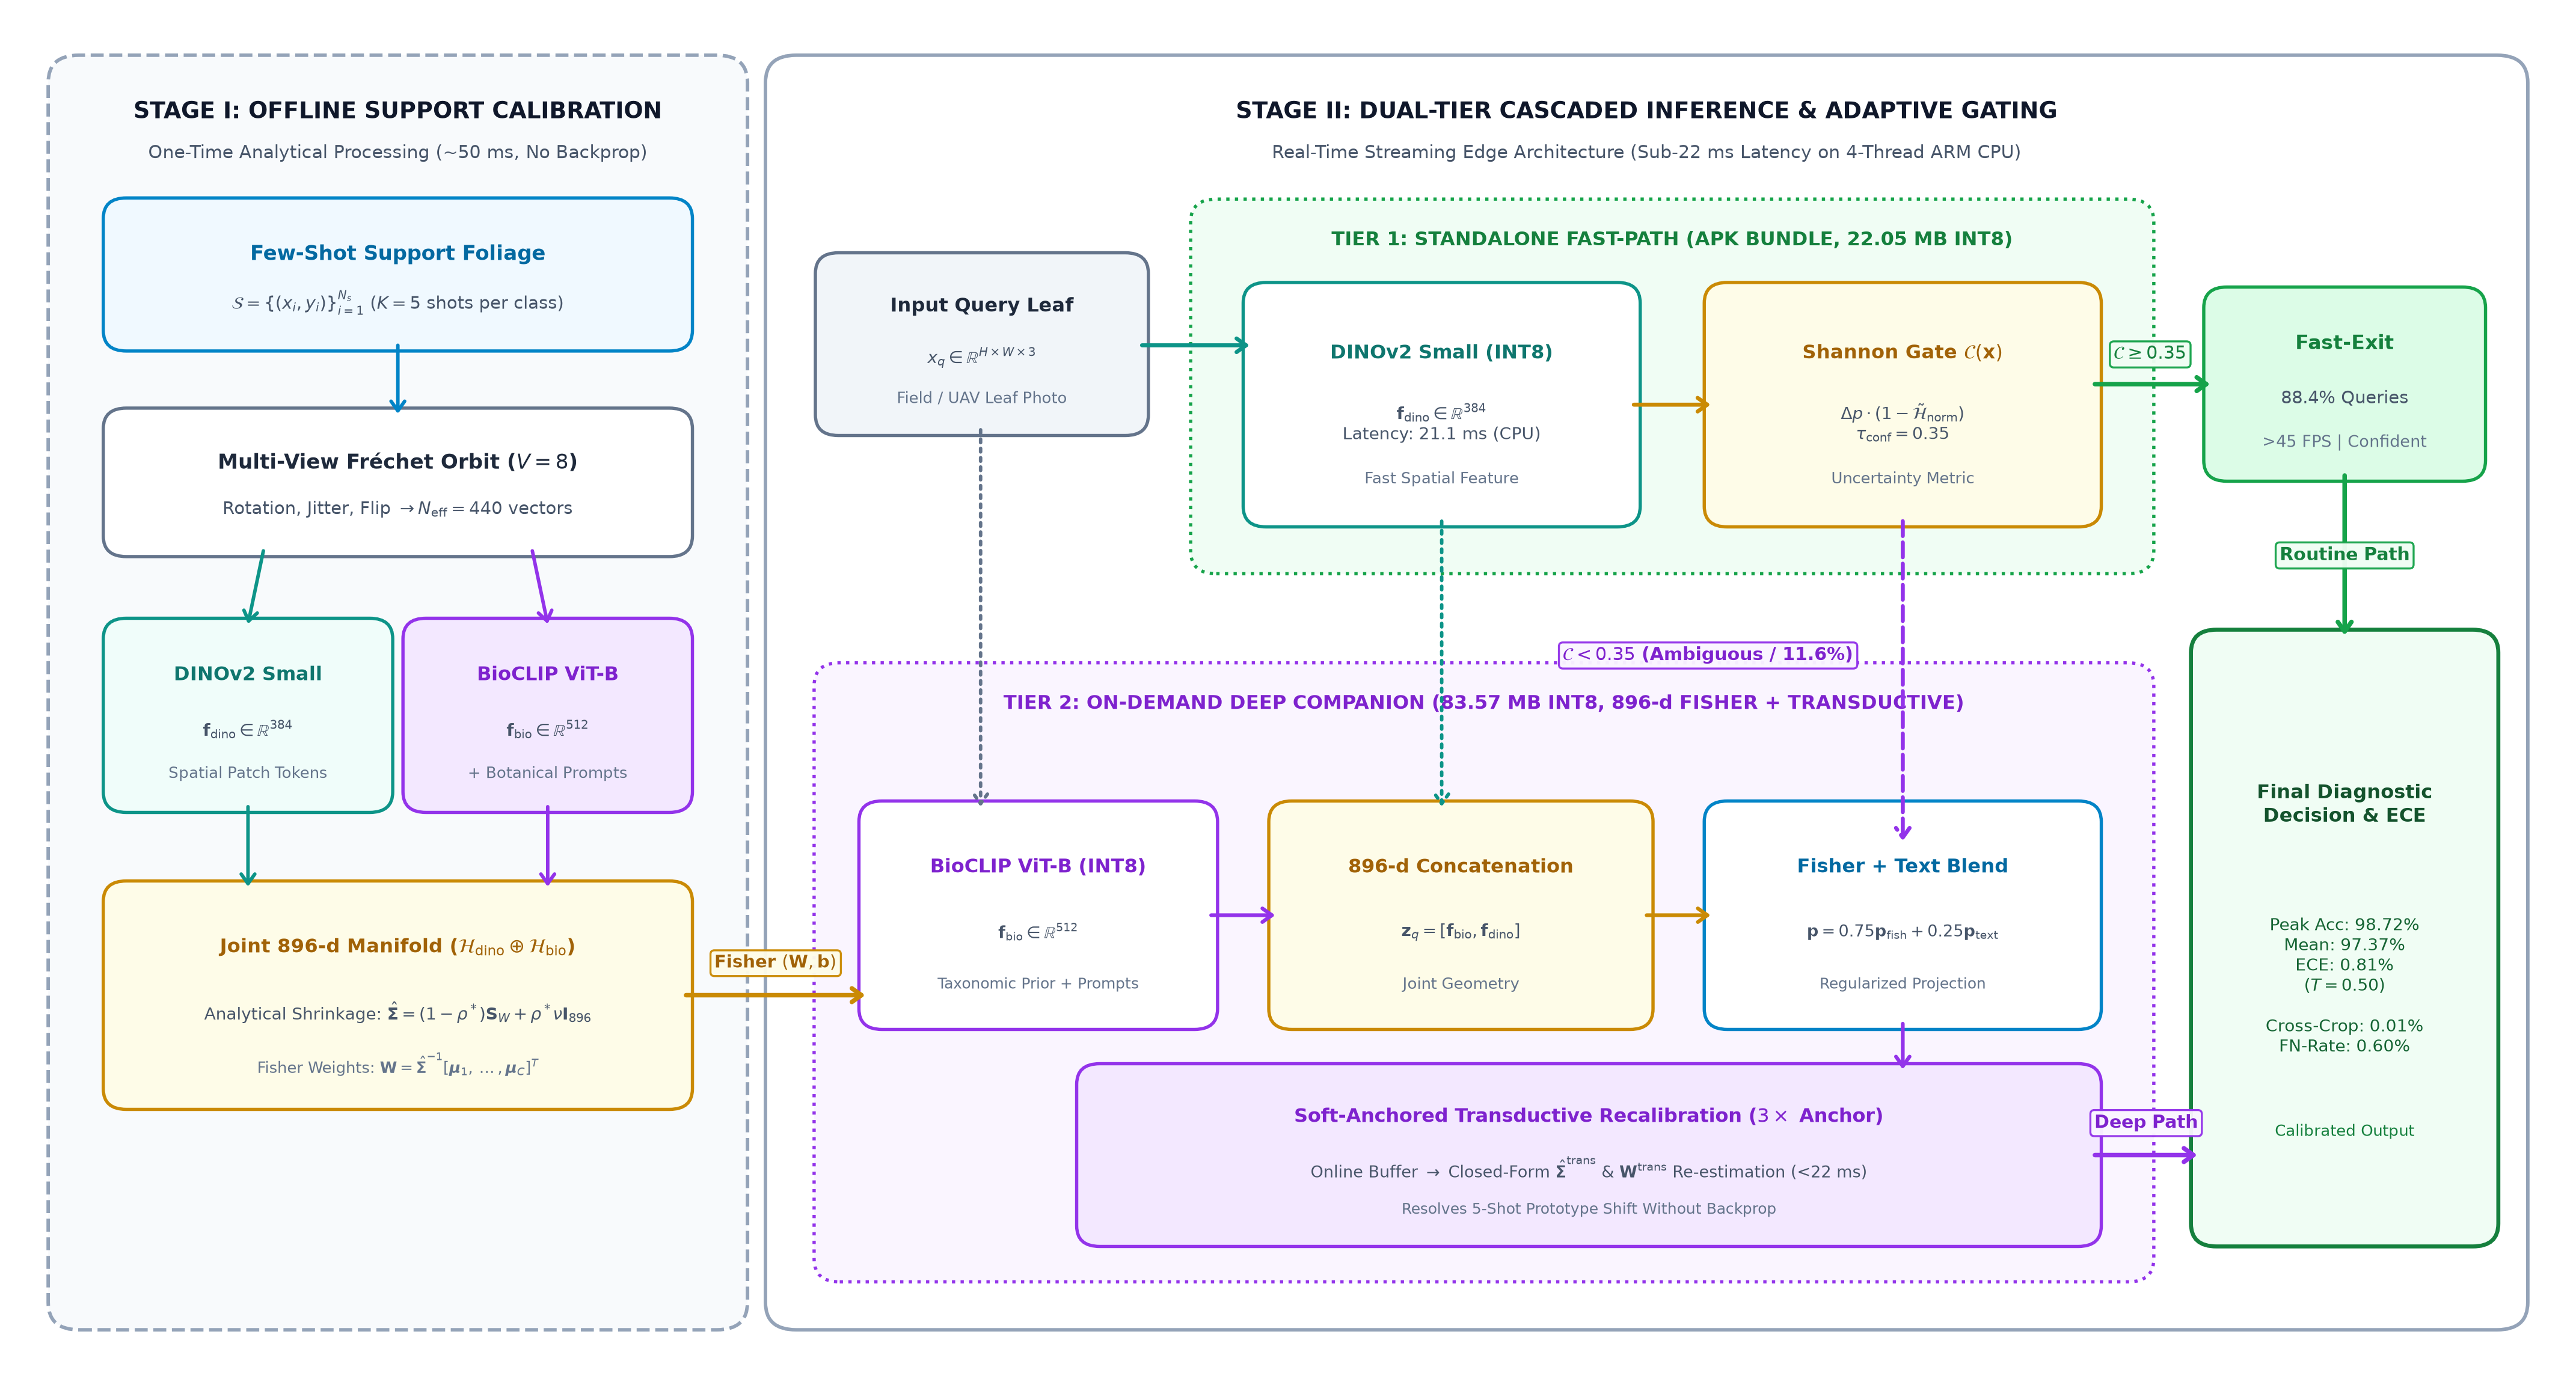
\includegraphics[width=\textwidth,height=4.2cm]{figures/fig_architecture.png}
    \caption{Architectural pipeline of the proposed MorphoPath-Edge diagnostic framework. Stage 1: Unconstrained agricultural imagery is ingested under complex field noise (glare, occlusions, soil clutter). Stage 2: Dual-stream frozen foundation backbones decouple macroscopic foliar organ geometry ($z_{\mathrm{dino}} \in \mathbb{R}^{384}$) from microscopic lesion pathology ($z_{\mathrm{bio}} \in \mathbb{R}^{512}$). Stage 3: Concatenated embeddings undergo Tukey power normalization and Zero-Parameter Test-Time Manifold Rectification (Proposition 1), canceling environmental domain translation $\Delta$ algebraically in 0.041\,ms. Stage 4: Geometric features drive the 4-Archetype Router, while intra-archetype subspaces are regularized via Ledoit--Wolf covariance shrinkage ($\lambda=0.60$) and combined with micro-symptom prompt ensembles. Stage 5: Cardinality-Equalized Bayesian Differential Triage corrects partition size bias, producing calibrated Top-1 and Top-2 clinical candidates.}
    \label{fig:architecture}
\end{figure*}

\subsection{Botanical Foliar Macro-Archetypes}
\label{subsec:foliar_macro_archetypes}
To eliminate cascading species-routing failures without collapsing into flat metric confusion, we introduce an architectural decomposition grounded in evolutionary botany and conserved leaf morphological phenotypes (Fig.~\ref{fig:archetypes}). We define a surjective mapping $\pi: \mathcal{Y} \to \mathcal{A}$, projecting the fine-grained label space $\mathcal{Y}$ onto four disjoint macroscopic foliar archetypes $\mathcal{A} = \{A_0, A_1, A_2, A_3\}$:
\begin{enumerate}[\IEEEsetlabelwidth{A3}\setlength{\itemsep}{0.5pt}\setlength{\parsep}{0pt}\setlength{\topsep}{1.5pt}]
    \item \textbf{Archetype $A_0$ (Solanoid -- Compound Dentate Lamina):} Solanaceous crops (\textit{Solanum lycopersicum} [Tomato], \textit{Solanum tuberosum} [Potato]). Morphologically characterized by imparipinnate compound foliage with dentate-to-serrate leaflet margins and reticulate secondary venation ($C_{A_0} = 10$ classes in PlantDoc).
    \item \textbf{Archetype $A_1$ (Vitoid -- Palmate Lobed Lamina):} Vitaceae and Cucurbitaceae (\textit{Vitis vinifera} [Grape], \textit{Cucurbita pepo} [Squash]). Defined by broad, actinodromous palmate venation radiating from the petiole junction with cordate, multi-lobed leaf bases ($C_{A_1} = 3$ classes in PlantDoc).
    \item \textbf{Archetype $A_2$ (Pooid -- Monocotyledonous Parallel Lamina):} Monocot grasses (\textit{Zea mays} [Corn]). Defined by elongated, strap-like blades with striate parallel venation lacking reticulate cross-vein networks ($C_{A_2} = 3$ classes in PlantDoc).
    \item \textbf{Archetype $A_3$ (Rosoid -- Simple Elliptical Lamina):} Rosaceae and perennial woody dicots (Apple, Peach, Cherry, Bell Pepper, Strawberry, Blueberry, Raspberry, Soybean). Characterized by simple, ovate-to-elliptical lamina with craspedodromous or camptodromous pinnate secondary venation ($C_{A_3} = 11$ classes in PlantDoc).
\end{enumerate}

The full label space decomposes into disjoint subsets: $\mathcal{Y} = \bigcup_{k=0}^3 \mathcal{Y}_{A_k}$, where $\mathcal{Y}_{A_k} = \{c \in \mathcal{Y} \mid \pi(c) = A_k\}$ and $\mathcal{Y}_{A_k} \cap \mathcal{Y}_{A_j} = \emptyset$ ($\forall k \ne j$). This reformulates 27-way field classification into a hierarchical Bayesian decision process:
\begin{equation}
    P(c \mid x) = P(\pi(c) \mid x) \cdot P_{\text{loc}}(c \mid x, \pi(c)),
    \label{eq:hierarchical_bayes_base}
\end{equation}
where $P(\pi(c) \mid x)$ denotes the macroscopic foliar archetype prior, and $P_{\text{loc}}(c \mid x, \pi(c))$ represents localized intra-archetype pathological likelihood.